%                                                                 aa.dem
% AA vers. 8.2, LaTeX class for Astronomy & Astrophysics
% demonstration file
%                                                       (c) EDP Sciences
%-----------------------------------------------------------------------
%
%\documentclass[referee]{aa} % for a referee version
%\documentclass[onecolumn]{aa} % for a paper on 1 column  
%\documentclass[longauth]{aa} % for the long lists of affiliations 
%\documentclass[rnote]{aa} % for the research notes
%\documentclass[letter]{aa} % for the letters 
%\documentclass[bibyear]{aa} % if the references are not structured 
% according to the author-year natbib style

%
\documentclass{aa}  

%
\usepackage{graphicx}
%%%%%%%%%%%%%%%%%%%%%%%%%%%%%%%%%%%%%%%%
\usepackage{txfonts}
%%%%%%%%%%%%%%%%%%%%%%%%%%%%%%%%%%%%%%%%
%\usepackage[options]{hyperref}
% To add links in your PDF file, use the package "hyperref"
% with options according to your LaTeX or PDFLaTeX drivers.
%
\begin{document} 


   \title{Analysis of the formation of Massive Globular Clusters after a Galaxy Merge}

%   \subtitle{Analysis of the formation of Massive Globular Clusters after a Galaxy Merge}

   \author{Paula Cáceres Burgos}

   \institute{Departamento de Astronomía, Universidad de Chile. \\
              \email{paula.caceres.burgos@gmail.com}
             }

   \date{Received April 22, 2019}

% \abstract{}{}{}{}{} 
% 5 {} token are mandatory
 
  \abstract
  % context heading (optional)
  % {} leave it empty if necessary  
  % {To investigate the physical nature of the `nuc\-leated instability' of
   %proto giant planets, the stability of layers
   %in static, radiative gas spheres is analysed on the basis of Baker's
   %standard one-zone model.}
  % aims heading (mandatory)
   %{It is shown that stability
   %depends only upon the equations of state, the opacities and the local
   %thermodynamic state in the layer. Stability and instability can
   %therefore be expressed in the form of stability equations of state
   %which are universal for a given composition.}
  % methods heading (mandatory)
   %{The stability equations of state are
   %calculated for solar composition and are displayed in the domain
   %$-14 \leq \lg \rho / \mathrm{[g\, cm^{-3}]} \leq 0 $,
   %$ 8.8 \leq \lg e / \mathrm{[erg\, g^{-1}]} \leq 17.7$. These displays
   %may be
   %used to determine the one-zone stability of layers in stellar
   %or planetary structure models by directly reading off the value of
   %the stability equations for the thermodynamic state of these layers,
   %specified
   %by state quantities as density $\rho$, temperature $T$ or
   %specific internal energy $e$.
   %Regions of instability in the $(\rho,e)$-plane are described
   %and related to the underlying microphysical processes.}
  % results heading (mandatory)
   %{Vibrational instability is found to be a common phenomenon
   %at temperatures lower than the second He ionisation
   %zone. The $\kappa$-mechanism is widespread under `cool'
   %conditions.}
  % conclusions heading (optional), leave it empty if necessary 
   %{}

   \keywords{galaxies: star clusters --
                %$\kappa$-mechanism --
                %stability of gas spheres
               }

   \maketitle
%
%________________________________________________________________

%que es un cumulo globular 
%cuales son las condiciones para que ocurran
%relacionar lo anterior con el choque de galaxias 

%porque es importante saber 


\section{Introduction}

   
   Massive Globular Clusters \textbf{(MGCs)} are the lagest and most masive star clusters known in the universe. Their name comes from having a very symmetrical and somewhat spherical form.\\
   However, when it comes to knowing how MGCs form we must rely on various theories. Some of them being the collapse of a protogalaxy (S. Michael Fall \& Martin J. Rees, 1985), of a supergiant molecular cloud \textbf{(SGMC)} (William E. Harris \& Ralph E. Pudritz, 1994), the high pressure of the ISM of starbursts combined with a high star formation efficiency in giant molecular clouds \textbf{(GMCs)} (Keith M. Ashman \& Stephen E. Zepf, 2001) and the vigorous star forming regions that starbursts and galaxy mergers provide (Keith M. Ashman \& Stephen E. Zepf, 1998). In this report we will focus in the latter, where there is evidence of MGC formation in rotationally supported disks in merging galaxies (Escala, A. \& Larson. B, 2008).\\ Supported by the simulation of GADGET-2 and studying the instabilities of the disks of the galaxy merge, we expect to predict which regions of the latter will ultimately convert into a MGC and to characterize them. 
   We start going into more detail about GADGET-2 in $\S2$. In $\S3$ we study the instability of the disk, to later calculate the parameters needed in $\S4$ for a simulated Milky Way type Galaxy to ensure the attainment of reliable measurements; then in $\S5$  we do the same as in $\S4$ but with a galaxy merge simulation. Finally in $\S6$ we enunciate our conclusions.

\section{GADGET-2 Simulator}
   GADGET-2 is a cosmological simulation that evolves self-gravitating collisionless fluids with the traditional N-body approach, and a collisional gas by smoothed particle hydrodynamics (V. Springel, N. Yoshidaa, S. D.M. White., 2001). 
 
\section{Instabilities of the disk}
   For a uniformly rotating disk, the dispersion relation for small perturbations is given by:
   \begin{equation}
       \omega^2 = 4\Omega^2 - 2\pi G \Sigma\mid k \mid + k^2C_{s}^2
   \end{equation}
   (Binney \& Tremaine, 1987) Where $C_S$ is the speed of light,  G is the gravitational constant, $\Sigma$ is the surface density, $\Omega$ is the angular rotation speed and k is the wave number.
   Studying the stabilities of (1) we obtain that for the extreme case of $\Omega$ being zero we have an inferior limit for the wavelength of the system, while for $C_s = 0$ we have a superior one. These constraints are called $\lambda_{jeans}$ and $\lambda_{rot}$ respectively, whose values are:\\
   \begin{equation}
       \lambda_{jeans} = C_s^2/ G \Sigma_{gas}
   \end{equation}
   \begin{equation}
       \lambda_{rot} = \pi^2 G \Sigma_{gas} / \Omega^2 
   \end{equation}
   These values also have an associated mass, that are defined by: 
   \begin{equation}
       M_{jeans} = \Sigma_{gas}(\lambda_{jeans}/2)^2 = \frac{C_s^4}{4 G^2 \Sigma_{gas}}
   \end{equation}
   \begin{equation}
       M_{rot} = \Sigma_{gas}(\lambda_{rot}/2)^2 = \frac{\pi^4 G^2 \Sigma_{gas}^3}{4 \Omega^4}
   \end{equation}
   Having these limits we know that for wavelengths (masses) lesser than $\lambda_{jeans}$ ($M_{jeans}$) and greater than $\lambda_{rot}$ ($M_{rot}$) the disk is stable, so we observe that the instabilities are associated with the range of wavelengths between $\lambda_{jeans}$ ($M_{jeans}$) and $\lambda_{rot}$ ($M_{rot}$). So for us to assure the stability of the disk, we must shrink to zero the range of  $\lambda_{jeans}$ and $\lambda_{rot}$ by determining a relation between both of these values. This relation is firstly determined by Toomre (1964), who enunciates that for the range to be shrunken $\lambda_{jeans} \geqslant \lambda_{rot}/4$ must be satisfied; and along this relation, a criterion of stability is derived:

   \begin{equation}
        \mid Q \mid \equiv \frac{C_S \mid \Omega \mid}{G \Sigma_{gas}} 
   \centering
   \end{equation}
   where $\Sigma_{gas}$ is the density gas surface. This criterion is defined in such a way that for $Q \geqslant 1$ the disk is stable, and for $Q < 1$ it's unstable. However when it comes to studying the disks of merging galaxies is unwise for us to approximate it to a uniform rotating disk, when we know the chaoticness occurring in those situations. Therefore, in order to use this criterion more rigorously, Escala (2013) proposes a new criterion: 
   

 %  Many of the galaxy mergers happening in the universe are places of current massive cluster formation (Escala et al. 2013). Therefore these spots can be characterized as a constant collapse of Giant Molecular Clouds (GMC). However for the latter to ultimately become a Massive Globular Cluster (GC) (with mass up to $10^5 - 10^6 M_{\odot}$) not only does it require to be very massive but also to have an important star formation efficiency. We assume that a combination of both takes place.\\
%   Taking in consideration that star formation efficiency is directly linked to the study of the instability of gas (that later translates to the fragmentation of it, and the genesis of the star), we begin considering our system of merging galaxies as one of a rotating disk and proceed to analyze it's instability. Relating these concepts, Escala (2013) proposes an instability criterion:
   \begin{equation}
        \mid Q_0 \mid \equiv \frac{C_S \mid \Omega_{0} \mid}{G \Sigma_{gas}} \geqslant q
   \centering
   \end{equation}
   \begin{equation}
       \Omega_{0} = \frac{r \times v }{r^2} = \hat{r} \times \frac{v}{r}
   \end{equation}
   Where  $\mid\Omega_0\mid$ is the norm of the generalized angular velocity and q is a normalization constant. Hence the new relation that must be satisfied for the wavelengths are $\lambda_{jeans} \geqslant (q/\pi)^2 \lambda_{rot}$; and analogous to Toomre's criterion, for $\mid \Omega_0 \mid / q  \geqslant 1$ the merging disk will be stable, and for $\mid \Omega_0 \mid / q  < 1$ it will be unstable.\\
   Having all these relations well defined we will mainly concentrate on verifying that the mass of the regions of gas that will later convert to star clusters are at all time between the lower and upper limits of $M_{jeans}$ and $M_{rot}$. And after that, we expect to characterize those regions to understand the matter that makes a region collapse into a MGC. 
   
  
   \section{Galaxy Simulation}
   Considering the purpose of this report, we must assure that we calculate properly all the parameters needed for $M_{rot}$ and $M_{jeans}$. Therefore with GADGET-2 we simulate a Milky Way type galaxy centered in the x-y plane with an exponential density profile truncated at a certain radius to compare our computed calculations to the ones that GADGET-2 provides us. \\
   \begin{figure}[h!]
   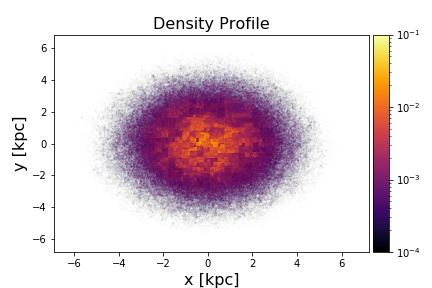
\includegraphics[scale=0.55]{Galaxy.png}
   \caption{}
   \centering
   \label{fig:boat1}
   \end{figure}
   The parameters to be calculated are $C_s$, $\Omega_0$ and $\Sigma_{gas}$.\\ To be continued are the explanation of how we did it.
   \subsection{Calculating $C_s$}
   The formula used for the speed of sound is: 
   \begin{equation}
       C_s = \sqrt{\gamma (\gamma - 1) u}
   \end{equation}
   Where $\gamma$ are the degrees of freedom and $u$ is the internal energy. This calculation is easily computed for every particle of the simulation thanks to the information provided by GADGET-2.  
   \subsection{Calculating $\Omega_0$}
   The formula used for this calculation was equation (8). Here we computed all the positions $(x,y,z)$ of the gas particles and all the components of the velocity $(v_x, v_y, v_z)$ to calculate $\Omega_0$, and because of the symmetry, we also considered the ideal angular velocity $\Omega$ as:
   \begin{equation}
       r = \sqrt{x^2 + y^2}
   \end{equation}
   \begin{equation}
       v = \sqrt{v_x^2 + v_y^2}
   \end{equation}
   \begin{equation}
       \Omega = v/r
   \end{equation}
   to compare it's values. The results are shown in Fig. 2.
   
   \subsection{Calculating $\Sigma_{gas}$}
   Determining the values of the density surface of the gas is quite more complicated. Firstly we computed the theoretical value of the density surface. Since we know it's an exponential fit, we consider: 
   \begin{equation}
       \Sigma_{theo} = \Sigma_0 \exp{(-r/r_d)}
   \end{equation}
   with $\Sigma_0$ estimated as 0.015 and $r_d$ as 1. Next we begin computing our own density surface with two methods: the first one consisting of taking the surface area of the x-y plane determined by Delaunay Tessellation and the mass of the gas particles (which is a constant) to find the density gas surface:
   \begin{equation}
       \Sigma_{tes} = (D+1) M_{gas}/A_{tes}
   \end{equation}
   where D is the dimension in which we are making the calculations (D=2) (F. I. Pelupessy, W. E. Schaap, and R. van de Weygaert, 2003).
   While the second one consists on using concentric annulus in the x-y plane to calculate the contained mass and area in them (using equation 15). 
   \begin{equation}
       \Sigma_{calc} = M_{gas}/A_{calc}
   \end{equation}
   The results are shown in Fig. 3. 
   \begin{figure}[h!]
   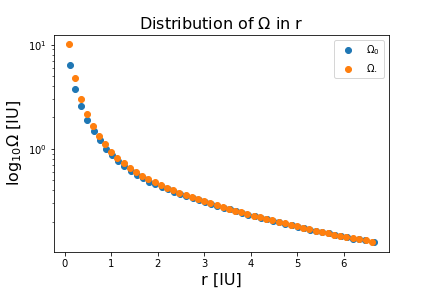
\includegraphics[scale=0.55]{Distribution_w.png}
   \caption{Distribution of the angular velocity along the radius of the Milky Way type Galaxy. The orange dotted line is the ideal angular velocity and the blue one is the generalized angular velocity.}
   \centering
   \label{fig:boat1}
   \end{figure}
   
   
   \begin{figure}[h]
   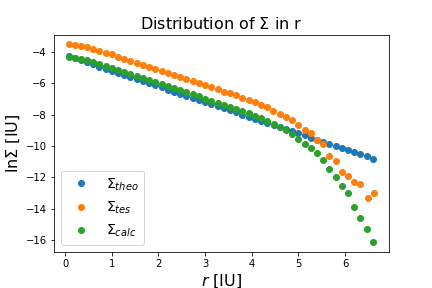
\includegraphics[scale=0.55]{Distribution_sigma_par_tot.png}
   \caption{Distribution of density surfaces along the radius. The blue dotted line shows the theoretical density surface, while the orange and green dotted line are the tessellated and calculated density surface respectively.}
   \centering
   \label{fig:boat1}
   \end{figure}
   
   \section{Merge Simulation}
   For the merge simulation we use two disk type galaxies that collide on a 90 degree angle, and we let this system evolve until we discern well formed star clumps (which is around the 76th timestep). Considering the star formation process and the id generator that GADGET-2 has internally configured, we must retrieve the progenitor particles of the star clumps and follow their evolution along all the timesteps, determining their $M_{rot}$ and $M_{jeans}$ at all time. \\
   We find the progenitor particles by taking the id's of a clump of the 76th timestep and compare it to the id's of the first timestep, keeping in track which of those repeat and which could be the potential "parent" or "grandparent" according to GADGET-2's configuration.  
   Once we have the progenitors, we begin calculating the parameters $\Sigma_{gas}$, $C_s$ and $\Omega_0$ for every snapshot, being very cautious specially with  $\Sigma_{gas}$ because the chaotic dynamics of a galaxy merge produces the so called $streams$, which makes a lot more harder to calculate a surface density (this is observed in fig.4 and fig.5). \\
   The way to compute $\Sigma_{gas}$ of a region is to calculate it's angular momentum, so we can determine the predominant axis of rotation, to later calculate the density surface of the plane perpendicular to it
   \begin{figure}[h!]
   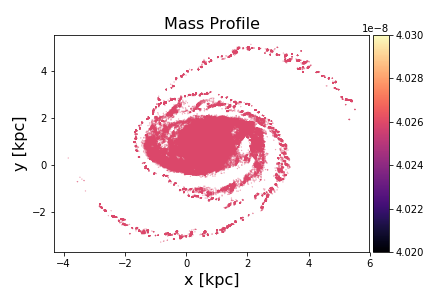
\includegraphics[scale=0.55]{Distribution_masa.png}
   \caption{The Mass Profile of the stars in the x-y plane at the 76th timestep. We can observe various distinguishable clumps in the "arms" of the merge (these are the streams)}
   \centering
   \label{fig:boat1}
   \end{figure}
   \begin{figure}[h!]
   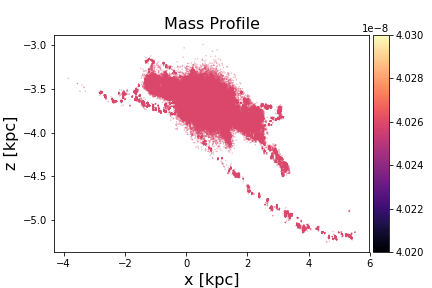
\includegraphics[scale=0.55]{Distribution_masa_delao.png}
   \caption{The Mass Profile of the stars in the x-z plane at the 76th timestep. Here, we can grasp how complex it is to calculate $\Sigma_{gas}$ since the merge can not be constrained to the x-y plane.}
   \centering
   \label{fig:boat1}
   \end{figure}
   Unfortunately, because of time and other difficulties it wasn't possible to compute correctly the $\Sigma_{gas}$ value for all the timesteps, leading to not being able to verify the reliability of the upper and lower limits of $M_{rot}$ and $M_{jeans}$. 
   
   %can lead ultimatelly to the genesis of Massive Globular Clusters, but in reality this is hard to achieve. 

%__________________________________________________________________


\section{Conclusions}

%   \begin{enumerate}
%      \item The conditions for the stability of static, radiative
%         layers in gas spheres, as described by Baker's (\cite{baker})
%         standard one-zone model, can be expressed as stability
%         equations of state. These stability equations of state depend
%         only on the local thermodynamic state of the layer.
%      \item If the constitutive relations -- equations of state and
%       Rosseland mean opacities -- are specified, the stability
%         equations of state can be evaluated without specifying
%         properties of the layer.
%      \item For solar composition gas the $\kappa$-mechanism is
%         working in the regions of the ice and dust features
%         in the opacities, the $\mathrm{H}_2$ dissociation and the
%         combined H, first He ionization zone, as
%         indicated by vibrational instability. These regions
%         of instability are much larger in extent and degree of
%         instability than the second He ionization zone
%         that drives the Cephe{\"\i}d pulsations.
%   \end{enumerate}

\begin{acknowledgements}
      %Part of this work was supported by the German
      %\emph{Deut\-sche For\-schungs\-ge\-mein\-schaft, DFG\/} project
      %number Ts~17/2--1.
      This work was importantly supported by Juan Molina, who guided me through the right path  
\end{acknowledgements}


%-------------------------------------------------------------------

\begin{thebibliography}{}

  \bibitem[2008]{Escala & Larson} Escala, A., \& Larson, B., 2008 \\
      Stability of Galactic Gas Disks and the Formation of Massive Clusters
      

   \bibitem[2013]{Escala et. al} Escala et. al, 2013\\
      Gravitational Fragmentation in Galaxy Mergers: A Stability Criterion
      
   \bibitem[2001]{Springel, Yoshidaa, & White.} V. Springel, N. Yoshidaa, S. D.M. White., 2001 \\
      GADGET: a code for collisionless and gasdynamical cosmological simulations

  % \bibitem[1980]{cox} Cox, J. P. 1980,
   %   Theory of Stellar Pulsation
    %  (Princeton University Press, Princeton) 165

   %\bibitem[1969]{cox69} Cox, A. N.,\& Stewart, J. N. 1969,
    %  Academia Nauk, Scientific Information 15, 1

   %\bibitem[1980]{mizuno} Mizuno H. 1980,
    %  Prog. Theor. Phys., 64, 544
   
   %\bibitem[1987]{tscharnuter} Tscharnuter W. M. 1987,
    %  A\&A, 188, 55
  
   %\bibitem[1992]{terlevich} Terlevich, R. 1992, in ASP Conf. Ser. 31, 
    %  Relationships between Active Galactic Nuclei and Starburst Galaxies, 
    %  ed. A. V. Filippenko, 13

   %\bibitem[1980a]{yorke80a} Yorke, H. W. 1980a,
     % A\&A, 86, 286

   %\bibitem[1997]{zheng} Zheng, W., Davidsen, A. F., Tytler, D. \& Kriss, G. A.
    %  1997, preprint
\end{thebibliography}

\end{document}

%%%%%%%%%%%%%%%%%%%%%%%%%%%%%%%%%%%%%%%%%%%%%%%%%%%%%%%%%%%%%%
Examples for figures using graphicx
A guide "Using Imported Graphics in LaTeX2e"  (Keith Reckdahl)
is available on a lot of LaTeX public servers or ctan mirrors.
The file is : epslatex.pdf 
%%%%%%%%%%%%%%%%%%%%%%%%%%%%%%%%%%%%%%%%%%%%%%%%%%%%%%%%%%%%%%

%_____________________________________________________________
%                 A figure as large as the width of the column
%-------------------------------------------------------------
   \begin{figure}
   \centering
   \includegraphics[width=\hsize]{empty.eps}
      \caption{Vibrational stability equation of state
               $S_{\mathrm{vib}}(\lg e, \lg \rho)$.
               $>0$ means vibrational stability.
              }
         \label{FigVibStab}
   \end{figure}
%
%_____________________________________________________________
%                                    One column rotated figure
%-------------------------------------------------------------
   \begin{figure}
   \centering
   \includegraphics[angle=-90,width=3cm]{empty.eps}
      \caption{Vibrational stability equation of state
               $S_{\mathrm{vib}}(\lg e, \lg \rho)$.
               $>0$ means vibrational stability.
              }
         \label{FigVibStab}
   \end{figure}
%
%_____________________________________________________________
%                        Figure with caption on the right side 
%-------------------------------------------------------------
   \begin{figure}
   \sidecaption
   \includegraphics[width=3cm]{empty.eps}
      \caption{Vibrational stability equation of state
               $S_{\mathrm{vib}}(\lg e, \lg \rho)$.
               $>0$ means vibrational stability.
              }
         \label{FigVibStab}
   \end{figure}
%
%_____________________________________________________________
%
%_____________________________________________________________
%                                Figure with a new BoundingBox 
%-------------------------------------------------------------
   \begin{figure}
   \centering
   \includegraphics[bb=10 20 100 300,width=3cm,clip]{empty.eps}
      \caption{Vibrational stability equation of state
               $S_{\mathrm{vib}}(\lg e, \lg \rho)$.
               $>0$ means vibrational stability.
              }
         \label{FigVibStab}
   \end{figure}
%
%_____________________________________________________________
%
%_____________________________________________________________
%                                      The "resizebox" command 
%-------------------------------------------------------------
   \begin{figure}
   \resizebox{\hsize}{!}
            {\includegraphics[bb=10 20 100 300,clip]{empty.eps}
      \caption{Vibrational stability equation of state
               $S_{\mathrm{vib}}(\lg e, \lg \rho)$.
               $>0$ means vibrational stability.
              }}
         \label{FigVibStab}
   \end{figure}
%
%______________________________________________________________
%
%_____________________________________________________________
%                                             Two column Figure 
%-------------------------------------------------------------
   \begin{figure*}
   \resizebox{\hsize}{!}
            {\includegraphics[bb=10 20 100 300,clip]{empty.eps}
      \caption{Vibrational stability equation of state
               $S_{\mathrm{vib}}(\lg e, \lg \rho)$.
               $>0$ means vibrational stability.
              }}
         \label{FigVibStab}
   \end{figure*}
%
%______________________________________________________________
%
%_____________________________________________________________
%                                             Simple A&A Table
%_____________________________________________________________
%
\begin{table}
\caption{Nonlinear Model Results}             % title of Table
\label{table:1}      % is used to refer this table in the text
\centering                          % used for centering table
\begin{tabular}{c c c c}        % centered columns (4 columns)
\hline\hline                 % inserts double horizontal lines
HJD & $E$ & Method\#2 & Method\#3 \\    % table heading 
\hline                        % inserts single horizontal line
   1 & 50 & $-837$ & 970 \\      % inserting body of the table
   2 & 47 & 877    & 230 \\
   3 & 31 & 25     & 415 \\
   4 & 35 & 144    & 2356 \\
   5 & 45 & 300    & 556 \\ 
\hline                                   %inserts single line
\end{tabular}
\end{table}
%
%_____________________________________________________________
%                                             Two column Table 
%_____________________________________________________________
%
\begin{table*}
\caption{Nonlinear Model Results}             
\label{table:1}      
\centering          
\begin{tabular}{c c c c l l l }     % 7 columns 
\hline\hline       
                      % To combine 4 columns into a single one 
HJD & $E$ & Method\#2 & \multicolumn{4}{c}{Method\#3}\\ 
\hline                    
   1 & 50 & $-837$ & 970 & 65 & 67 & 78\\  
   2 & 47 & 877    & 230 & 567& 55 & 78\\
   3 & 31 & 25     & 415 & 567& 55 & 78\\
   4 & 35 & 144    & 2356& 567& 55 & 78 \\
   5 & 45 & 300    & 556 & 567& 55 & 78\\
\hline                  
\end{tabular}
\end{table*}
%
%-------------------------------------------------------------
%                                          Table with notes 
%-------------------------------------------------------------
%
% A single note
\begin{table}
\caption{\label{t7}Spectral types and photometry for stars in the
  region.}
\centering
\begin{tabular}{lccc}
\hline\hline
Star&Spectral type&RA(J2000)&Dec(J2000)\\
\hline
69           &B1\,V     &09 15 54.046 & $-$50 00 26.67\\
49           &B0.7\,V   &*09 15 54.570& $-$50 00 03.90\\
LS~1267~(86) &O8\,V     &09 15 52.787&11.07\\
24.6         &7.58      &1.37 &0.20\\
\hline
LS~1262      &B0\,V     &09 15 05.17&11.17\\
MO 2-119     &B0.5\,V   &09 15 33.7 &11.74\\
LS~1269      &O8.5\,V   &09 15 56.60&10.85\\
\hline
\end{tabular}
\tablefoot{The top panel shows likely members of Pismis~11. The second
panel contains likely members of Alicante~5. The bottom panel
displays stars outside the clusters.}
\end{table}
%
% More notes
%
\begin{table}
\caption{\label{t7}Spectral types and photometry for stars in the
  region.}
\centering
\begin{tabular}{lccc}
\hline\hline
Star&Spectral type&RA(J2000)&Dec(J2000)\\
\hline
69           &B1\,V     &09 15 54.046 & $-$50 00 26.67\\
49           &B0.7\,V   &*09 15 54.570& $-$50 00 03.90\\
LS~1267~(86) &O8\,V     &09 15 52.787&11.07\tablefootmark{a}\\
24.6         &7.58\tablefootmark{1}&1.37\tablefootmark{a}   &0.20\tablefootmark{a}\\
\hline
LS~1262      &B0\,V     &09 15 05.17&11.17\tablefootmark{b}\\
MO 2-119     &B0.5\,V   &09 15 33.7 &11.74\tablefootmark{c}\\
LS~1269      &O8.5\,V   &09 15 56.60&10.85\tablefootmark{d}\\
\hline
\end{tabular}
\tablefoot{The top panel shows likely members of Pismis~11. The second
panel contains likely members of Alicante~5. The bottom panel
displays stars outside the clusters.\\
\tablefoottext{a}{Photometry for MF13, LS~1267 and HD~80077 from
Dupont et al.}
\tablefoottext{b}{Photometry for LS~1262, LS~1269 from
Durand et al.}
\tablefoottext{c}{Photometry for MO2-119 from
Mathieu et al.}
}
\end{table}
%
%-------------------------------------------------------------
%                                       Table with references 
%-------------------------------------------------------------
%
\begin{table*}[h]
 \caption[]{\label{nearbylistaa2}List of nearby SNe used in this work.}
\begin{tabular}{lccc}
 \hline \hline
  SN name &
  Epoch &
 Bands &
  References \\
 &
  (with respect to $B$ maximum) &
 &
 \\ \hline
1981B   & 0 & {\it UBV} & 1\\
1986G   &  $-$3, $-$1, 0, 1, 2 & {\it BV}  & 2\\
1989B   & $-$5, $-$1, 0, 3, 5 & {\it UBVRI}  & 3, 4\\
1990N   & 2, 7 & {\it UBVRI}  & 5\\
1991M   & 3 & {\it VRI}  & 6\\
\hline
\noalign{\smallskip}
\multicolumn{4}{c}{ SNe 91bg-like} \\
\noalign{\smallskip}
\hline
1991bg   & 1, 2 & {\it BVRI}  & 7\\
1999by   & $-$5, $-$4, $-$3, 3, 4, 5 & {\it UBVRI}  & 8\\
\hline
\noalign{\smallskip}
\multicolumn{4}{c}{ SNe 91T-like} \\
\noalign{\smallskip}
\hline
1991T   & $-$3, 0 & {\it UBVRI}  &  9, 10\\
2000cx  & $-$3, $-$2, 0, 1, 5 & {\it UBVRI}  & 11\\ %
\hline
\end{tabular}
\tablebib{(1)~\citet{branch83};
(2) \citet{phillips87}; (3) \citet{barbon90}; (4) \citet{wells94};
(5) \citet{mazzali93}; (6) \citet{gomez98}; (7) \citet{kirshner93};
(8) \citet{patat96}; (9) \citet{salvo01}; (10) \citet{branch03};
(11) \citet{jha99}.
}
\end{table*}
%_____________________________________________________________
%                      A rotated Two column Table in landscape  
%-------------------------------------------------------------
\begin{sidewaystable*}
\caption{Summary for ISOCAM sources with mid-IR excess 
(YSO candidates).}\label{YSOtable}
\centering
\begin{tabular}{crrlcl} 
\hline\hline             
ISO-L1551 & $F_{6.7}$~[mJy] & $\alpha_{6.7-14.3}$ 
& YSO type$^{d}$ & Status & Comments\\
\hline
  \multicolumn{6}{c}{\it New YSO candidates}\\ % To combine 6 columns into a single one
\hline
  1 & 1.56 $\pm$ 0.47 & --    & Class II$^{c}$ & New & Mid\\
  2 & 0.79:           & 0.97: & Class II ?     & New & \\
  3 & 4.95 $\pm$ 0.68 & 3.18  & Class II / III & New & \\
  5 & 1.44 $\pm$ 0.33 & 1.88  & Class II       & New & \\
\hline
  \multicolumn{6}{c}{\it Previously known YSOs} \\
\hline
  61 & 0.89 $\pm$ 0.58 & 1.77 & Class I & \object{HH 30} & Circumstellar disk\\
  96 & 38.34 $\pm$ 0.71 & 37.5& Class II& MHO 5          & Spectral type\\
\hline
\end{tabular}
\end{sidewaystable*}
%_____________________________________________________________
%                      A rotated One column Table in landscape  
%-------------------------------------------------------------
\begin{sidewaystable}
\caption{Summary for ISOCAM sources with mid-IR excess 
(YSO candidates).}\label{YSOtable}
\centering
\begin{tabular}{crrlcl} 
\hline\hline             
ISO-L1551 & $F_{6.7}$~[mJy] & $\alpha_{6.7-14.3}$ 
& YSO type$^{d}$ & Status & Comments\\
\hline
  \multicolumn{6}{c}{\it New YSO candidates}\\ % To combine 6 columns into a single one
\hline
  1 & 1.56 $\pm$ 0.47 & --    & Class II$^{c}$ & New & Mid\\
  2 & 0.79:           & 0.97: & Class II ?     & New & \\
  3 & 4.95 $\pm$ 0.68 & 3.18  & Class II / III & New & \\
  5 & 1.44 $\pm$ 0.33 & 1.88  & Class II       & New & \\
\hline
  \multicolumn{6}{c}{\it Previously known YSOs} \\
\hline
  61 & 0.89 $\pm$ 0.58 & 1.77 & Class I & \object{HH 30} & Circumstellar disk\\
  96 & 38.34 $\pm$ 0.71 & 37.5& Class II& MHO 5          & Spectral type\\
\hline
\end{tabular}
\end{sidewaystable}
%
%_____________________________________________________________
%                              Table longer than a single page  
%-------------------------------------------------------------
% All long tables will be placed automatically at the end, after 
%                                        \end{thebibliography}
%
\begin{longtab}
\begin{longtable}{lllrrr}
\caption{\label{kstars} Sample stars with absolute magnitude}\\
\hline\hline
Catalogue& $M_{V}$ & Spectral & Distance & Mode & Count Rate \\
\hline
\endfirsthead
\caption{continued.}\\
\hline\hline
Catalogue& $M_{V}$ & Spectral & Distance & Mode & Count Rate \\
\hline
\endhead
\hline
\endfoot
%%
Gl 33    & 6.37 & K2 V & 7.46 & S & 0.043170\\
Gl 66AB  & 6.26 & K2 V & 8.15 & S & 0.260478\\
Gl 68    & 5.87 & K1 V & 7.47 & P & 0.026610\\
         &      &      &      & H & 0.008686\\
Gl 86 
\footnote{Source not included in the HRI catalog. See Sect.~5.4.2 for details.}
         & 5.92 & K0 V & 10.91& S & 0.058230\\
\end{longtable}
\end{longtab}
%
%_____________________________________________________________
%                              Table longer than a single page
%                                             and in landscape 
%  In the preamble, use:       \usepackage{lscape}
%-------------------------------------------------------------
% All long tables will be placed automatically at the end, after
%                                        \end{thebibliography}
%
\begin{longtab}
\begin{landscape}
\begin{longtable}{lllrrr}
\caption{\label{kstars} Sample stars with absolute magnitude}\\
\hline\hline
Catalogue& $M_{V}$ & Spectral & Distance & Mode & Count Rate \\
\hline
\endfirsthead
\caption{continued.}\\
\hline\hline
Catalogue& $M_{V}$ & Spectral & Distance & Mode & Count Rate \\
\hline
\endhead
\hline
\endfoot
%%
Gl 33    & 6.37 & K2 V & 7.46 & S & 0.043170\\
Gl 66AB  & 6.26 & K2 V & 8.15 & S & 0.260478\\
Gl 68    & 5.87 & K1 V & 7.47 & P & 0.026610\\
         &      &      &      & H & 0.008686\\
Gl 86
\footnote{Source not included in the HRI catalog. See Sect.~5.4.2 for details.}
         & 5.92 & K0 V & 10.91& S & 0.058230\\
\end{longtable}
\end{landscape}
\end{longtab}
%
% Online Material
%_____________________________________________________________
%        Online appendices have to be placed at the end, after
%                                        \end{thebibliography}
%-------------------------------------------------------------
%\end{thebibliography}

\Online

\begin{appendix} %First online appendix
\section{Background galaxy number counts and shear noise-levels}
Because the optical images used in this analysis...

\begin{figure*}
\centering
\includegraphics[width=16.4cm,clip]{1787f24.ps}
\caption{Plotted above...}
\label{appfig}
\end{figure*}

Because the optical images...
\end{appendix}

\begin{appendix} %Second online appendix
These studies, however, have faced...
\end{appendix}

%\end{document}
%
%_____________________________________________________________
%        Some tables or figures are in the printed version and
%                      some are only in the electronic version
%-------------------------------------------------------------
%
% Leave all the tables or figures in the text, at their right place 
% and use the commands \onlfig{} and \onltab{}. These elements
% will be automatically placed at the end, in the section
% Online material.

\documentclass{aa}
...
\begin{document}
text of the paper...
\begin{figure*}%f1
\includegraphics[width=10.9cm]{1787f01.eps}
\caption{Shown in greyscale is a...}
\label{cl12301}
\end{figure*}
...
from the intrinsic ellipticity distribution.
% Figure 2 available electronically only
\onlfig{
\begin{figure*}%f2
\includegraphics[width=11.6cm]{1787f02.eps}
\caption {Shown in greyscale...}
\label{cl1018}
\end{figure*}
}

% Figure 3 available electronically only
\onlfig{
\begin{figure*}%f3
\includegraphics[width=11.2cm]{1787f03.eps}
\caption{Shown in panels...}
\label{cl1059}
\end{figure*}
}

\begin{figure*}%f4
\includegraphics[width=10.9cm]{1787f04.eps}
\caption{Shown in greyscale is...}
\label{cl1232}
\end{figure*}

\begin{table}%t1
\caption{Complexes characterisation.}\label{starbursts}
\centering
\begin{tabular}{lccc}
\hline \hline
Complex & $F_{60}$ & 8.6 &  No. of  \\
...
\hline
\end{tabular}
\end{table}
The second method produces...

% Figure 5 available electronically only
\onlfig{
\begin{figure*}%f5
\includegraphics[width=11.2cm]{1787f05.eps}
\caption{Shown in panels...}
\label{cl1238}
\end{figure*}
}

As can be seen, in general the deeper...
% Table 2 available electronically only
\onltab{
\begin{table*}%t2
\caption{List of the LMC stellar complexes...}\label{Properties}
\centering
\begin{tabular}{lccccccccc}
\hline  \hline
Stellar & RA & Dec & ...
...
\hline
\end{tabular}
\end{table*}
}

% Table 3 available electronically only
\onltab{
\begin{table*}%t3
\caption{List of the derived...}\label{IrasFluxes}
\centering
\begin{tabular}{lcccccccccc}
\hline \hline
Stellar & $f12$ & $L12$ &...
...
\hline
\end{tabular}
\end{table*}
}
\end{document}
%
%-------------------------------------------------------------
%     For the online material, table longer than a single page
%                 In the preamble for landscape case, use : 
%                                          \usepackage{lscape}
%-------------------------------------------------------------
\documentclass{aa}
\usepackage[varg]{txfonts}
\usepackage{graphicx}
\usepackage{lscape}

\begin{document}
text of the paper
% Table will be print automatically at the end, in the section Online material.
\onllongtab{
\begin{longtable}{lrcrrrrrrrrl}
\caption{Line data and abundances ...}\\
\hline
\hline
Def & mol & Ion & $\lambda$ & $\chi$ & $\log gf$ & N & e &  rad & $\delta$ & $\delta$ 
red & References \\
\hline
\endfirsthead
\caption{Continued.} \\
\hline
Def & mol & Ion & $\lambda$ & $\chi$ & $\log gf$ & B & C &  rad & $\delta$ & $\delta$ 
red & References \\
\hline
\endhead
\hline
\endfoot
\hline
\endlastfoot
A & CH & 1 &3638 & 0.002 & $-$2.551 &  &  &  & $-$150 & 150 &  Jorgensen et al. (1996) \\                    
\end{longtable}
}% End onllongtab

% Or for landscape, large table:

\onllongtab{
\begin{landscape}
\begin{longtable}{lrcrrrrrrrrl}
...
\end{longtable}
\end{landscape}
}% End onllongtab
\end{document}